\documentclass{prova}

\usepackage{amsmath}
\usepackage{amsfonts}

\setlength{\textheight}{25cm}

\DeclareMathOperator{\sen}{sen}
\newcommand{\ds}{\displaystyle}

\professor{Prof.\@ Adriano Barbosa}
\disciplina{C\'alculo Diferencial e Integral}
\avaliacao{Final}
\curso{Engenharia de Produção}
\data{08/06/2021}

\begin{document}
	\cabecalho{5}  % o numero 5 indica a qnt de quadros na tabela de nota

    \textbf{Todas as respostas devem ser justificadas.}

    \begin{questionario}
        \q{Se $\ds\lim_{x\rightarrow a} \left[f(x)+g(x)\right]=-3$ e
            $\ds\lim_{x\rightarrow a} \left[f(x)-g(x)\right]=2$, encontre
            $\ds\lim_{x\rightarrow a} \left[f(x)g(x)\right]$.}
        \q{Seja $r$ a reta tangente à elipse $\ds\frac{x^2}{4} + \frac{y^2}{9}
            = 1$ num ponto $P$ do primeiro quadrante. Sejam $x_t$ e $y_t$ as
            interseções de $r$ com os eixos $x$ e $y$, respectivamente. À
            medida que $P$ se movimenta no primeiro quadrante sem tocar os
            eixos coordenados, o que podemos dizer sobre os valores de $x_t$ e
            $y_t$?}
            \begin{figure}[!h]
                \centering
                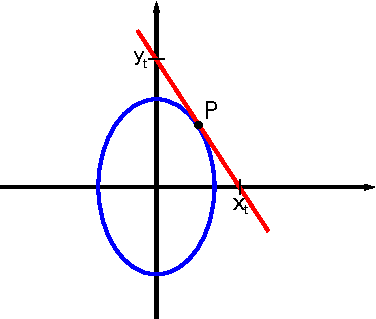
\includegraphics[width=0.3\textwidth]{elipse.pdf}
            \end{figure}
        \q{É possível encontrar uma função tal que $f'(0)=1$, $f'(1)=0$ e que
            $f''(x)>0$ para todo $x\in\mathbb{R}$? Exiba a função ou prove que
            não existe.}
        \q{Sejam $f(x) = \ds\int_0^{\sen{x}} 1+\cos{\left(t^2\right)}\ dt$ e $g(x) =
            \ds\int_0^{f(x)} \frac{x^2}{\sqrt{1+t^3}}\ dt$. Calcule $g'(\pi)$.}
    \end{questionario}
\end{document}
